\documentclass[letterpaper, 10 pt, conference]{ieeeconf}  % Comment this line out
                                                   % if you need a4paper
%\documentclass[a4paper, 10pt, conference]{ieeeconf}      % Use this line for a4

% paper
\usepackage{authblk}
\usepackage{graphicx}
\usepackage{esvect}
\usepackage{fancyhdr} 
\usepackage[section]{placeins}
\usepackage{float}
\usepackage{lipsum}
\IEEEoverridecommandlockouts                              % This command is only
\renewcommand\headrule{}                                                            % needed if you want to
                                                         % use the \thanks command
\overrideIEEEmargins

% See the \addtolength command later in the file to balance the column lengths
% on the last page of the document



% The following packages can be found on http:\\www.ctan.org
%\usepackage{graphics} % for pdf, bitmapped graphics files
%\usepackage{epsfig} % for postscript graphics files
%\usepackage{mathptmx} % assumes new font selection scheme installed
%\usepackage{times} % assumes new font selection scheme installed
%\usepackage{amsmath} % assumes amsmath package installed
%\usepackage{amssymb}  % assumes amsmath package installed

\title{\LARGE \bf
Automated Classification of Bug Fixes using Pattern Mining
}

\author{Kehkashan Fazal, Pooja Janagal Nagaraja and Rupa Mahadevan}% <-this 
% stops a spacehttps://www.overleaf.com/project/5c0efe93fe269a5444c37fba


\begin{document}

 

\maketitle

%%%%%%%%%%%%%%%%%%%%%%%%%%%%%%%%%%%%%%%%%%%%%%%%%%%%%%%%%%%%%%%%%%%%%%%%%%%%%%%%
\begin{abstract}

The goal of this project is to analyze the sentiment of Yelp reviews and classify them as positive or negative. We introduce feature extraction methods specific to users with the aim to account for the user's style of vocabulary usage and use these to learn models for all users. With Adaboost, classification accuracy of 87.46\% was obtained, which was observed to be comparable with that of conventional sentiment analysis techniques. 

\end{abstract}

%%%%%%%%%%%%%%%%%%%%%%%%%%%%%%%%%%%%%%%%%%%%%%%%%%%%%%%%%%%%%%%%%%%%%%%%%%%%%%%%
\section{Introduction}

In recent years, the explosion of social networking sites (e.g., Facebook, Twitter), blogs (e.g., Mashable, Techcrunch), and online review portals (e.g., Amazon, TripAdvisor, IMDB) has provided us with an overwhelming amount of information about products and services. Millions of people express uninhibited opinions about various product (or, service) features, and their nuances. As consumers cannot test the functionality of a product (or, service) prior to consumption, these reviews help them make an informed decision to buy the product (or, service). This begs the question, how important are reviews to customers and businesses in terms of sales?\\

According to a study \cite{c1}, 90\% of customers read online reviews before visiting a business, 88\% of customers trust the reviews as much as personal recommendations. 92\% users will use a local business with a more positive review, while customers spend 31\% more on a business with an "excellent" review. The power of social media and the new-age "word-of-mouth" has driven much research into this topic to tap into its full potential . \\

\textit{Sentiment analysis} is one such topic of research. Sentiment Analysis (also known as Opinion Mining) is a field within \textit{Natural Language Processing (NLP)} that builds systems that try to identify and extract opinions within text. With unstructured data ubiquitously available over the inter-webs in the form of reviews by users, sentiment analysis proves to be a powerful tool to make sense of these. \\

Being able to classify reviews to glean the sentiment of users for certain businesses can greatly boost sales and bring new user into their fray. It can also help local businesses decide their future policies. Better marketing strategies can also be devised, based on which part of the business the users like or dislike \cite{c2}. \\

One more important part of sentiment analysis that is often overlooked is the human-connect. Text used for sentiment-analysis is often not specific enough in regards to the users writing them. Just like the word "good" can indicate different degree of likability for different users, the degree of likability expressed in the review could potentially change from user to user for identical reviews.\\

In this paper, we address the above issues by encoding user information and general information, respectively, into two different models to generate two individual text representations with user attention or generalized analysis. \\

We generate not only a general, but also a user specific sentiment analysis and try to get the maximum accuracy possible. We have also used several models to do sentiment analysis and our aim is to evaluate which model performs the best for this task. 

\section{Data Description}

Our main focus for sentiment analysis will be on Yelp's review dataset. Yelp is a local-search service powered by crowd-sourced review forum with over 100 million reviews of almost every type of local business, from restaurants, boutiques and salons to dentists, mechanics, plumbers etc. It is because of this wide range of audience that Yelp is an ideal playground for sentiment analysts.\\ 

Yelp's Dataset has been sourced from the latest version of Yelp Dataset Challenge \cite{c3}. The reviews dataset is a file composed of a single object type, one JSON-object per-line. It contains full review text data including the user\_id that wrote the review and the business\_id the review is written for.\\

%\begin{figure}[htb]
%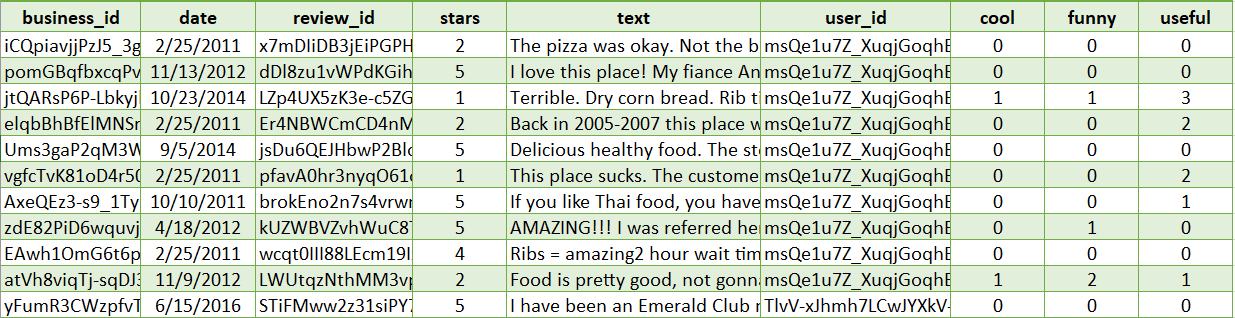
\includegraphics[height = 7cm, width = 9cm]{img/dataset.png}
%\caption{Snapshot of reviews.json}
%\label{fig:1}
%\end{figure}

The dataset contains 6 Million reviews given by 1.5 Million users for around 188595 businesses. For the purposes of this project, we have considered reviews with stars 1,2,4 and 5. Also, we only consider those users who have given 500 or more reviews for user-specific sentiment analysis to generate better accuracy across the user-specific models.\\

In Fig.~\ref{fig:1}, the first few rows of the dataset is shown. It is represented in .csv format after processing the JSON files and extracting the necessary data.

\begin{figure*}[htb]
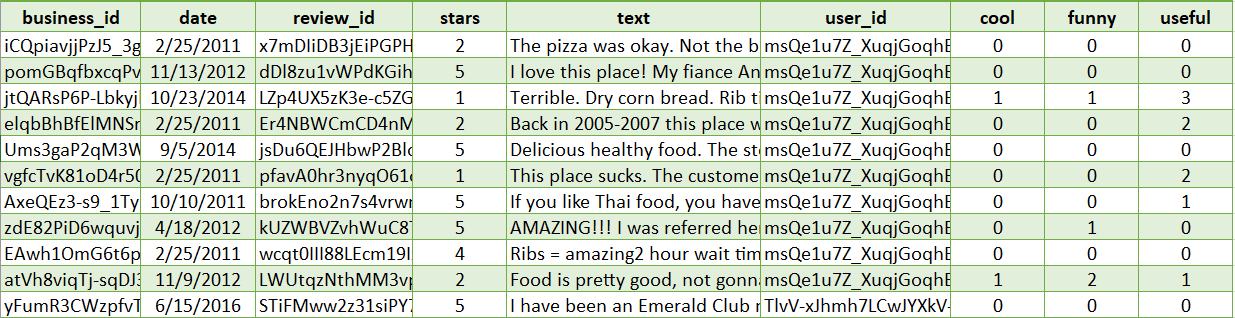
\includegraphics[height = 4cm, width=\textwidth]{img/dataset.png}
\caption{Example of rows in dataset} \label{fig:1}
\end{figure*}

\subsection{Data Exploration}

In this section, the data exploration in the project is presented with figures giving a rich insight of the data. These would also help in deciding the data pre-processing and feature extraction methods. Fig.~\ref{fig:2} shows the distribution of the stars across reviews. It can easily be seen that the data is highly unbalanced.

\begin{figure}[H]
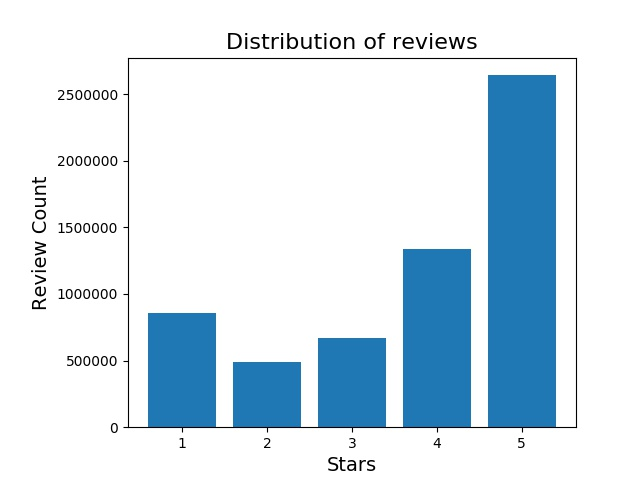
\includegraphics[width=\linewidth]{img/dist_reviews.jpg}
\caption{Distribution of stars over reviews} \label{fig:2}
\end{figure}

In Fig.~\ref{fig:3}, the distribution of average of stars per user is shown. We can see general spikes in both directions, with data neutralizing for more number of users.

\begin{figure}[htb]
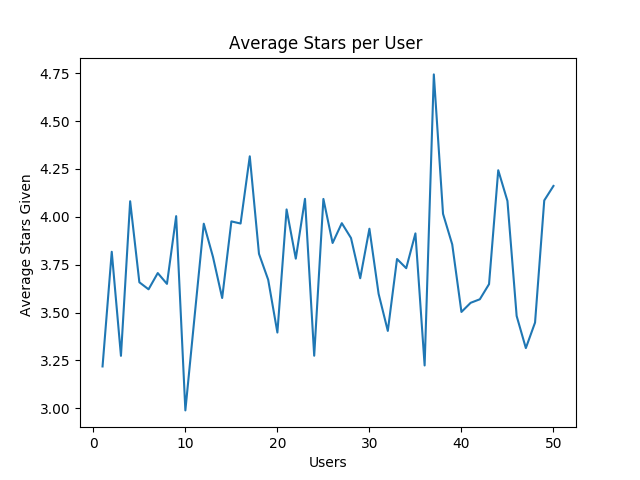
\includegraphics[ height = 5cm,width = \linewidth]{img/Average_per_user.png}
\caption{Average stars per user} \label{fig:3}
\end{figure}

In the Figure ~\ref{fig:4}, the \textit{histogram} of text length distributions for each star rating is shown. The distribution helps us decide which metrics would be best suited for sentiment analysis.\\

In the histogram, the 4 and 5 starred reviews generally have the highest word count. Positive reinforcements would thus be easy to learn from this dataset. It also points towards the probability that the dataset is more positively inclined as compared to negative examples that occur in the training dataset.\\

We decided to omit all 3-star reviews to more accurately balance our dataset and not include any ambiguous reviews that do not add value to the models.

\begin{figure}[htb]
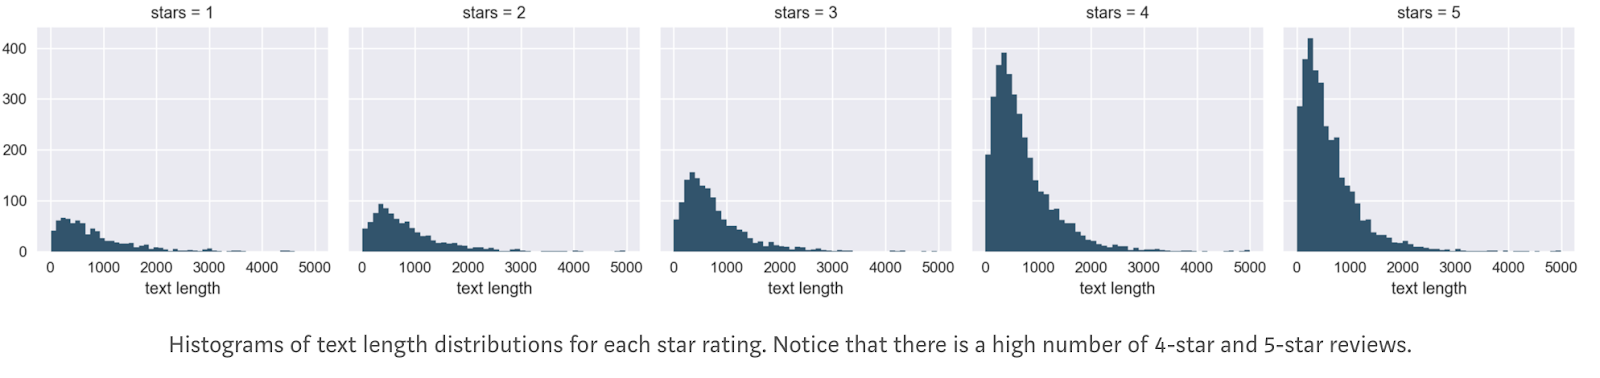
\includegraphics[width=\linewidth]{img/stars.png}
\caption{Histograms of text length distributions for each star rating}
\label{fig:4}
\end{figure}
In order to develop a user specific model, we decided to go with users who have reviewed establishments on Yelp more than 500 times. The reason for deciding this number stems from the data exploration and also from the belief that such users will tend to give more genuine reviews as compared to others. It will also help us test our model based on the particular style of that user so that we don't have to generalize the weights for a review word across all users.

\section{Methodology}

To perform both classic and user-specific sentiment analysis, a series of steps need to be followed. At first, various pre-processing methods were applied on the reviews. Features were extracted from these reviews and fed into the different models. These steps are crucial as they form the foundation of modelling.\\
\begin{enumerate}
\item {Data Pre-processing:} In this step, data is converted to .csv format, and standard approaches like stop-word removal, data cleaning etc. are employed along with approaches specific to our dataset, like selection of users and reviews to model user-specific sentiment analysis, removal of neutral reviews to create a more robust dataset and so on.\\
\item {Feature Extraction:} Here, we perform TF-IDF vectorization to extract the features. The classic method involves applying TF-IDF on the corpus of all reviews. Along with this, we also apply TF-IDF vectorization with respect to users. This user-specific approach gives us a better understanding of the importance of the words in a given user's language.\\
\item {Classification:} Finally, we choose different classifiers and train a model for each user. The accuracy is computed as a combination of accuracy measures across all the models. This accuracy is compared with the classification accuracy obtained from classic method which involves training one model for a given classifier.\\ 
\end{enumerate}
These processes are explained in further detail in the following sections.
The methodology used by us is also depicted in Figure ~\ref{fig:5}

\begin{figure}[htb]
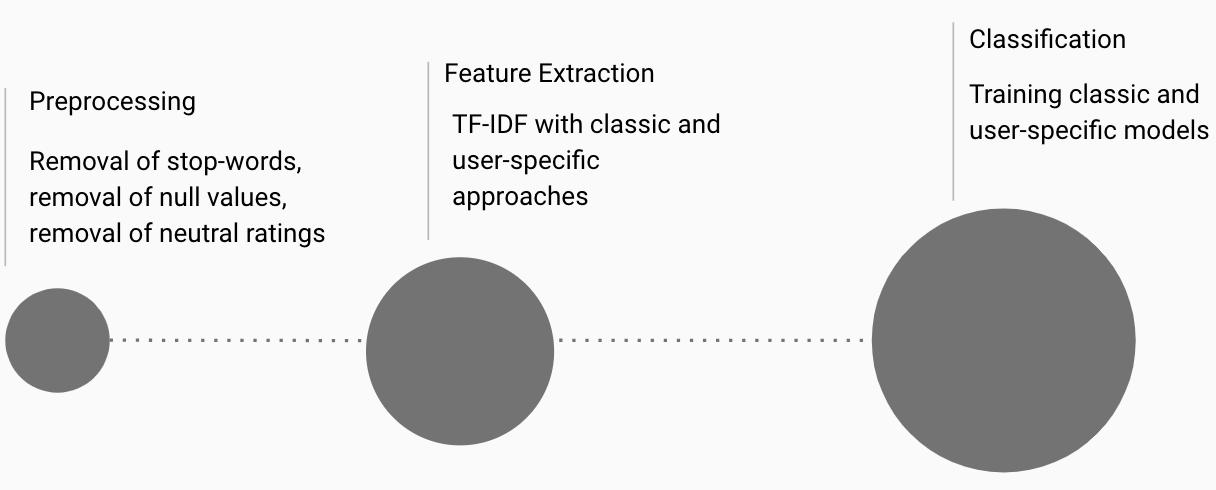
\includegraphics[width=\linewidth]{img/method.png}
\caption{Methodology}
\label{fig:5}
\end{figure}

\section{Data Pre-processing}

In this section, different data pre-processing techniques and data cleaning techniques are discussed. Few of these steps are the standard pre-processing procedures that need to be applied for any sentiment analysis and model building task \cite{c9}. Apart from these, we also apply a few methods specific to our dataset. This helps us in filtering out irrelevant information and preserving the most useful representation of the reviews. 

\subsection{Extraction of data from JSON format}

Yelp's dataset is provided in a JSON format. An example of the JSON file can be seen below in Figure.~\ref{fig:6}.\\
\begin{figure}[htb]
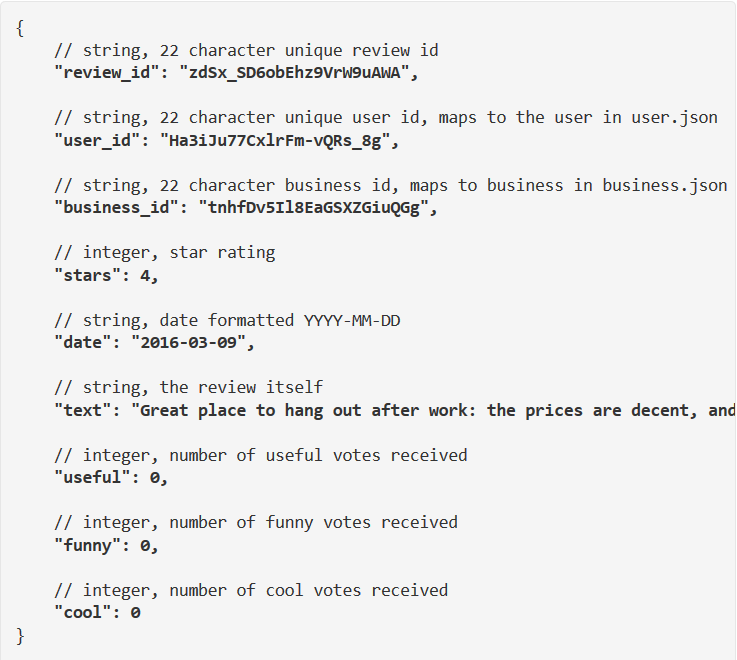
\includegraphics[width = \linewidth]{img/yelp_json.png}
\caption{JSON representation of data}
\label{fig:6}
\end{figure}

The following data attributes were gleaned from the dataset:
\begin{enumerate}
    \item business\_id: ID of the business being reviewed
    \item date: Day the review was posted
    \item review\_id: ID for the posted review
    \item stars: 1 to 5 rating for the business
    \item text: Review text
    \item user\_id: User’s ID
    \item \{cool / useful / funny\}: Comments on the review, given by other users.\\
\end{enumerate}
The JSON file is converted to CSV format to 
improve readability and make it compatible with programming tools. 


\subsection{Removal of Stop words}

Stop words are words that do not add any significance to the meaning of a sentence, but are frequently occurring. These words are extremely common and would have a very little value of their inclusion in the vocabulary. An example of a subset can be seen below in  Figure.~\ref{fig:8}.
\begin{figure}[htb]
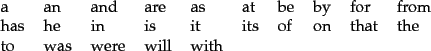
\includegraphics[width = \linewidth]{images/image8.png}
\caption{Examples of stop words}
\label{fig:8}
\end{figure}

\subsection{Spelling correction}

As the nature of online reviews is usually informal, the data is expected to contain spelling errors.
There are a few misspelled terms in the dataset, which are listed in Table I. It is crucial to correct the spellings as a consistent dataset for future analysis is necessary.

\begin{table}
\centering
\caption{Examples of wrong spellings}\label{tab1}
\begin{tabular}{|l|l|}
\hline
\textbf{Wrong Spelling} & \textbf{Correct Spelling} \\
\hline
Refrigerator & Refrigerator\\
\hline
Rechargeable & Rechargeable\\
\hline
Shoppe & Shop\\
\hline
Refrigerator & Refrigerator\\
\hline
\end{tabular}
\end{table}

\subsection{Removal of neutral reviews}

3 star reviews present a neutral sentiment and could be misclassified as positive or negative depending on the bias of the system. We thus decided to remove these reviews from the training set for the purposes of our experiment. Only reviews with 1 or 2 stars (negative) and 4 and 5 stars (positive) are retained in the dataset.

\subsection{Identification of users}

For user specific sentiment analysis, we needed a training set for each user with a considerable number of reviews, for the model to be able to identify the style in which the user writes his/her reviews. After data exploration, we decided to choose a subset of 50 users who have written greater than or equal to 500 reviews each.

\subsection{Preserving Useful Reviews}

The dataset contains 'useful' as one of the attributes. This is a rating given for a particular review by other users. Using this label, we can filter out the reviews that do not provide us with significant or new information. Also, using the 'date' attribute, we filter out outdated reviews.

\section{Feature Extraction}

The reviews cannot be directly used as features, as the dataset in this project does not translate to numerical features, but to textual data. Text data has to be converted to numerical vectors to fit the machine learning models.

\subsection{Methods to convert Text to Numerical Vectors}

\subsubsection{TF-IDF vectorization}

The reviews in the Yelp dataset cannot be directly used as features for the learning models as they represent textual data. Each review needs to be converted to a numerical vector. The models take in these numerical vectors as representation of reviews and learn from them. We have used TF-IDF for extracting features from reviews.
\\

\textit{tf–idf or TF-IDF}, short for term frequency–inverse document frequency is one of the most commonly used methods in \textit{Natural Language Processing}, where a given text would be converted to a corresponding vector, based on how important a given word is to the document. The value of TF-IDF increases proportionally to the number of times the word appears in the document and decreases by the number of documents in the corpus that contain that word. There are 2 quantities for every term in the vocabulary to be calculated. They are Term Frequency (TF) and Inverse Document Frequency (IDF) which would be defined below,\\

\noindent Let, \\
$x$ = Number of times term t occurs in document i\\
$y$ = Total Number of terms in the document i
\begin{equation}
TF = \frac{x}{y}
\end{equation}
Let, \\
$a$ = Total Number of Documents \\
$b$ = Total number of Documents containing term t

\begin{equation}
IDF = \ln{\frac{a}{b}}
\end{equation}

The TF-IDF feature for document $i$ and term $t$ would be $TF*IDF$. Hence a particular term can be represented as a vector of length equal to the number of documents, with the respective TF-IDF weights associated with it.\\


\subsubsection{User Specific TF-IDF vectorization}

When we use the classic method of applying TF-IDF over a corpus containing all the reviews, we do not take the difference in the language of different users into consideration. For instance, User1 uses the word 'good' in his/her reviews a lot more times than User2 does. User1 uses this positive word with much more liberty than User2. So the weights given to this particular word differs between the two users. This difference in treatment of words in the language is not reflected in the classic approach. Therefore, we experiment with a user-specific TF-IDF vectorization where TF-IDF is calculated independently for each user. The frequency is evaluated over the corpus of the reviews belonging to a particular user. In this approach, the difference in treatment of words is represented as TF-IDF for a given user is built only using his/her reviews. 

\section{Models}

\subsection{Multinomial Naive Bayes}

{Multinomial Naive Bayes} is a flavour of {Naive Bayes algorithm} \cite{c10}. Naive Bayes is a family of algorithms obtained by applying Bayes theorem with a strong(naive) assumption that every feature is independent of the others, in order to predict the category of a given sample. This is a probabilistic classifier, therefore will calculate the probability of each category using Bayes theorem, and the category with the highest probability will be the output of the classifier. Naive Bayes classifiers have been successfully applied to many domains, and has been known to perform well particularly in Natural Language Processing(NLP) applications. \\

With a multinomial event model, samples (feature vectors) represent the frequencies with which certain events have been generated by a multinomial $( p_1 , \dots , p_n )$ where $p_i$ is the probability that event $i$ occurs (or K such multinomials in the multiclass case). A feature vector ${x} =(x_{1},\dots ,x_{n})$ is then a histogram, with $x_{i}$ counting the number of times event $i$ was observed in a particular instance. This is the event model typically used for review classification, with events representing the occurrence of a word in a single document or in our case, the term frequency-inverse document frequency. The likelihood of observing a histogram $x$ is then given by:
\begin{center}
  ${\displaystyle p(\mathbf {x} \mid C_{k})={\frac {(\sum _{i}x_{i})!}{\prod _{i}x_{i}!}}\prod _{i}{p_{ki}}^{x_{i}}}$\\  
\end{center}

Multinomial Naive Bayes is a good model to start with, even though there exist many algorithms for coping with NLP problems. The simple design of Naive Bayes classifiers make them very attractive for such tasks. Moreover, they have been demonstrated to be fast, reliable and accurate in a number of applications of NLP. 

\subsection{Gradient Boosting}

{Gradient Boosting} is a machine learning technique for regression and classification problems \cite{c11}, which uses an ensemble of weak learners, typically like decision trees. It builds the model iteratively like other boosting methods do, and it generalizes them by optimization of an arbitrary differentiable loss function.  \\

It is easiest to explain gradient boosting in the least-squares regression setting, where the goal is to "teach" a model $F$ to predict values of the form $\hat {y}=F(x)$ by minimizing the mean squared error $\tfrac {1}{n}\sum _{i}({\hat {y}}_{i}-y_{i})^{2}$, where $i$ indexes over some training set of size $n$ of actual values of the output variable $y$.  \\

In the case of gradient boosting, the learning method successively fits new models to find a more accurate estimate of the class variable. Every new model is correlated with the negative gradient of the loss function and tends to minimize it. This is materialized by using the gradient descent method.\\

The goal is to find an approximation $\hat {F}(x)$ to a function$F(x)$ that minimizes the expected value of some specified loss function $L(y, F(x))$:

    $${\displaystyle {\hat {F}}={\underset {F}{\arg \min }}\,\mathbb {E} _{x,y}[L(y,F(x))]}.$$

The gradient boosting method assumes a real-valued y and seeks an approximation$\hat{F}(x)$ in the form of a weighted sum of functions $h_i (x)$ from some class $\mathcal {H}$, called base (or weak) learners:

   $$ {\displaystyle {\hat {F}}(x)=\sum _{i=1}^{M}\gamma _{i}h_{i}(x)+{\mbox{const}}}.$$
    
One of the most powerful characteristics that GBM has is its ability to use different types of base learners, like linear models, smooth models, decision trees, Markov models, etc. A list that categorizes the base learners is presented below:
\begin{enumerate}
    \item Linear models: ordinary linear regression, ridge penalized linear regression and random effects.
    \item Smooth models: P-splines, radial basis functions.
    \item Decision trees: decision tree stumps, decision trees with arbitrary interaction depth.
    \item Other cases of models: Markov random fields, custom base learner functions, wavelets.
\end{enumerate}

This feature provides the ability of one GBM to encompass more than one base learners. Additionally, GBM can cope with high-dimensional data due to its ability to create sparse models. This advantage is very useful in the case of sentiment analysis.\\

We thus applied Gradient Boosting on the TF-IDF vectors generated for both the classic and user specific sentiment analysis models. Being an ensemble technique, Gradient Boosting performed much better when compared for both accuracy and recall with Multinomial Naive Bayes.

\subsection{K-nearest Neighbor (KNN)}

The  K-Nearest  Neighbor  (KNN) \cite{c12}  is  one  of  the  simplest  lazy  machine  learning algorithms.  It is a supervised learning technique where the algorithm  classifies  objects  into  one  of  the  predefined classes  of  a  sample  group. KNN is based on finding the most similar objects (documents) from sample groups using a distance metric and evaluating the new unseen data into the same class as that of the maority its neighbours.\\

During the learning phase, the  algorithm determines  the  reviews  which  will  be  comparing  with  each  new  review. The  algorithm  assumes  that it  is  possible  to classify  documents  in  the  Euclidean  space  as  points.  Euclidean distance is the distance between two points in Euclidean space. The distance between two points in the plane with coordinates p=(x, y) and q=(a, b) can be calculated: 

$$ \begin{aligned}
        d(\mathbf {q} ,\mathbf {p} ) = {\sqrt {\sum _{i=1}^{n}(q_{i}-p_{i})^{2}}}
        \end{aligned} \\
$$
    
The K-nearest neighbours to a review can be computed using distance metrics other than Euclidean distance as well. Some of the popular distance metrics are Mahalanobis distance, Manhattan distance, Minkowski distance, etc. For the given dataset, we found that Euclidean distance was the best measure.\\

Another metric that KNN can be optimized on is the number of neighbours used for the classification. Using grid search and cross validation, 60 neighbours were chosen. The optimal K value is usually $\sqrt{n}$ , where n is the number of samples in the training dataset.\\

In  KNN  classification,  the  unknown  pattern  is assigned  the  most  predominant  class amongst  the  classes  of  its nearest neighbors. In case there is a tie between two classes for the pattern,  the  class  that  has  minimum  average  distance  to  the  unknown pattern is assigned. Through the combination of a number of local distance functions based on individual attributes, a global distance function dist can be calculated. 

\subsection{AdaBoost}

{AdaBoost} short for {Adaptive Boosting}, is a machine learning meta-algorithm used to improve the performance of the already existing weak classifiers. The output of the other learning algorithms ('weak learners') is combined into a weighted sum that represents the final output of the boosted classifier. AdaBoost is adaptive in the sense that subsequent weak learners are tweaked in favor of those instances misclassified by previous classifiers during the previous iterations.\\

AdaBoost refers to a particular method of training a boosted classifier. A boost classifier is a classifier in the form

    $$ F_T(x) = \sum_{t=1}^T f_t(x)$$

where each $f_{t}$ is a weak learner that takes a training $x$ as input and returns a value predicting the class of the object. For example, in the two class problem, the sign of the weak learner output identifies the predicted object class and the absolute value gives the confidence in that classification. Similarly, the $T$th classifier is positive if the sample is in the positive class and negative otherwise.\\

Each weak learner produces an output hypothesis, $h(x_i)$, for each sample in the training set. At each iteration $t$, a weak learner is selected and assigned a coefficient $\alpha_t$ so that the sum training error $E_{t}$ of the resulting $t$-stage boost classifier is minimized.

    $$E_t = \sum_i E[F_{t-1}(x_i) + \alpha_t h(x_i)]$$

Here $F_{t-1}(x)$ is the boosted classifier or strong classifier that has been built up to the previous stage of training,$E(F)$ is an error function and $\alpha_t h(x)$ is the weight of the weak learner that is being considered for addition to the final classifier. \\

At each iteration of the training process, a weight $w_{i,t}$ is assigned to each sample in the training set based on the current error$E(F_{t-1}(x_i))$ on that sample. These weights are used to pick a weak learner, for instance, decision trees, which can favor splitting sets of samples with high weights into its correct class. \\

During the training phase, we have to learn the functions $f_{i}$ with each containing the structure of the tree and the leaf scores. Unlike, the traditional optimization problem, this cannot be solved under gradient descent, rather we have to use an \textit{additive strategy}. \\

AdaBoost corresponds to a single iteration of the backfitting algorithm in which the smoothing splines are the minimizers of 
    $$\sum_{i=1}^n e^{-Y_i \hat\mu(x_i)} + \infty \int_{x_1}^{x_n} \hat\mu''(x)^2 \,dx$$,
    
that is: ${\hat {\mu }}_{i}$ fits an exponential cost function and is linear with respect to the observation.\\
 
At each step, the tree that optimizes the objective is chosen. The form of residual sum of squares of error can be used. However,the AdaBoost error function $E(f) = e^{-y(x)f(x)}$ takes into account the fact that only the sign of the final result is used, thus $|F(x)|$ can be far larger than 1 without increasing error. However, the exponential increase in the error for sample $x_{i}$ as $-y(x_i)f(x_i)$ increases results in excessive weight being assigned to outliers. \\

One feature of the choice of exponential error function is that the error of the final additive model is the product of the error of each stage, that is, $e^{\sum_i -y_i f(x_i)} = \prod_i e^{-y_i f(x_i)}$. Thus it can be seen that the weight update in the AdaBoost algorithm is equivalent to recalculating the error on $F_t(x)$ after each stage. \\

AdaBoost is being increasingly used as the best model for optimization and competitions in Kaggle. Unlike other powerful classifiers, such as SVM, AdaBoost can achieve similar classification results with much less tweaking of parameters or settings (unless of course you choose to use SVM with AdaBoost) \cite{c11}. The user only needs to choose: 
\begin{enumerate}
\item which weak classifier might work best to solve their given classification problem; 
\item the number of boosting rounds that should be used during the training phase. 
\end{enumerate}  \\

In our experiments as well, AdaBoost was the best performing model for user specific review analysis out of all the models that we tried. Its accuracy was comparable to that obtained using the classic review analysis model generated using Ada Boost.
\vspace{-2mm}
\section{Results}
The below are the performance measures obtained for different models. The metrics that have been considered to evaluate the different models used are: Accuracy, Precision, Recall and F1- Score \cite{c14}.\\

Accuracy is defined as the number of correct classifications over the total number of datapoints. While accuracy is a good metric to assess the performance of a model, it is not sufficient for evaluation when the data set is imbalanced, as in our case. In such scenarios, the precision, recall and F1 score give a good picture of the performance of the models. \\

Precision is the number of actual positive predictions to the total number of positive predictions made by the model. Recall is the number of true positives to the total number of data points that actually belong to the positive class. F1 score is used to combine precision and recall into one score for easier analysis and evaluation of the models. 

\begin{table}[H]
\begin{center}
 \caption{Performance Measures for Multinomial Naive Bayes}
  \begin{tabular}{ |c|c|c| }
    \hline
    \textbf{}&{\textbf{Classic}} & \textbf{User Specific}\\ \hline
    Accuracy & 88.7\% & 73.79\%\\ \hline
    Precision & 0.90 & 0.74\\ \hline 
    Recall & 0.98 & 1\\ \hline 
    F1 Score & 0.94 & 0.85\\ \hline 
    \hline
  \end{tabular}
\end{center}
\end{table}

Table II compares the performance of Multinomial Naive Bayes on the classic and user specific models. The accuracy of the user specific model is poor. However, the recall value of the classification model on user specific data becomes 1.

\begin{table}[H]
\begin{center}
 \caption{Performance Measures for Gradient Boosting}
  \begin{tabular}{ |c|c|c| }
    \hline
    \textbf{}&{\textbf{Classic}} & \textbf{User Specific}\\ \hline
    Accuracy & 89.5\% & 85.47\%\\ \hline
    Precision & 0.93 & 0.87\\ \hline 
    Recall & 0.85 & 0.94\\ \hline 
    F1 Score & 0.89 & 0.91\\ \hline 
    \hline
  \end{tabular}
\end{center}
\end{table}

Table III reports the performance of Gradient Boosting on sentiment analysis of the reviews. The table shows that the accuracy of Gradient Boosting on the classic and user specific models are comparable. The F1 score of the user specific model is better than that of the classic model.

\begin{table}[H]
\begin{center}
 \caption{Performance Measures for KNN }
  \begin{tabular}{ |c|c|c| }
    \hline
    \textbf{}&{\textbf{Classic}} & \textbf{User Specific}\\ \hline
    Accuracy & 90.1\% & 84.9\%\\ \hline
    Precision & 0.88 & 0.86\\ \hline 
    Recall & 0.97 & 0.95\\ \hline 
    F1 Score & 0.92 & 0.9\\ \hline 
    \hline
  \end{tabular}
\end{center}
\end{table}

Table IV reports the performance of KNN for classic and user specific models. The precision, recall and F1 scores of KNN is comparable between the classic and user specific models. The best model was obtained for Euclidean distance metric and 60 nearest neighbours.

\begin{table}[H]
\begin{center}
 \caption{Performance Measures for AdaBoost }
  \begin{tabular}{ |c|c|c| }
    \hline
    \textbf{}&{\textbf{Classic}} & \textbf{User Specific}\\ \hline
    Accuracy & 92.4\% & 87.46\%\\ \hline
    Precision & 0.96 & 0.89\\ \hline 
    Recall & 0.98 & 0.95\\ \hline 
    F1 Score & 0.97 & 0.92\\ \hline 
    \hline
  \end{tabular}
\end{center}
\end{table}

It can be seen from the above table that the gradient boosting models outperform other preliminary techniques. AdaBoost with Gradient Boosting Decision Tree has given the best results out of all the models experimented.

\section{CHALLENGES}
Following are some of the challenges we faced during this project:
\begin{itemize}
\item Storage requirements for user-specific analysis - As we are building a model for each user, these models need to be stored for predictions in the future. More the number of users involved , more is the storage requirement for all the trained models. 
\item Minimum requirements for reviews per user - We retain reviews from only those users who have posted greater than or equal to 500 reviews. Such a constraint poses a challenge which is hard to deal with when the data is not sufficient.
\item Identifying sarcasm, double negation and user extended vocabulary.\\
\end{itemize}
The main challenge of sentiment analysis remains tackling the nuance of a language. For example, the particular challenge of classifying these reviews:
\begin{itemize}
\item  I do not dislike the food here. \textit{(Negation handling)}
\item  Sometimes I really hate the ribs at this joint, but I keep coming back for more. \textit{(Adverbial modifies the sentiment)}
\item  Yes! Please keep us waiting for a salad for 30 mins. You know how much we love to sit and count tiles in this fine establishment. \textit{(Possibly sarcastic)}
\item  You should see their decadent dessert menu.\textit{ (Attitudinal term has shifted polarity recently in certain domains)}
\item  I love Fatburger but would not recommend it to any of my colleagues. \textit{(Qualified positive sentiment, difficult to categorise)}
\item  Yeet the sushi at this dumphole! \textit{(Newly minted terms can be highly attitudinal but volatile in polarity and often out of known vocabulary.)}
\end{itemize}

\section{FUTURE SCOPE}

We have identified the following modifications to the existing model to give richer results:
\begin{enumerate}
\item Combination of two TF-IDFs - The classic approach and user-specific approach can be combined to generate a much more powerful representation of the data.
\item Combining models of different users - We can combine models for users with similar language instead of building a model per user. This will drastically bring down the storage requirements. 
\item We can attempt to predict how genuine a particular user’s comment will be based on sentiment classification of past reviews by the same user.

\end{enumerate}


\section{CONCLUSIONS}

In this project, a very relevant challenge with regards to user specific and general sentiment analysis was tackled. Many features and meta-data were considered and various ways of achieving user centric sentiment analysis were touched upon. Numerous models were also experimented upon to provide a robust and highly accurate solution. The discussed approaches would perform very well on other sentiment analysis tasks as well.

\addtolength{\textheight}{-12cm}   % This command serves to balance the column lengths
                                  % on the last page of the document manually. It shortens
                                  % the textheight of the last page by a suitable amount.
                                  % This command does not take effect until the next page
                                  % so it should come on the page before the last. Make
                                  % sure that you do not shorten the textheight too much.

%%%%%%%%%%%%%%%%%%%%%%%%%%%%%%%%%%%%%%%%%%%%%%%%%%%%%%%%%%%%%%%%%%%%%%%%%%%%%%%%



%%%%%%%%%%%%%%%%%%%%%%%%%%%%%%%%%%%%%%%%%%%%%%%%%%%%%%%%%%%%%%%%%%%%%%%%%%%%%%%%



%%%%%%%%%%%%%%%%%%%%%%%%%%%%%%%%%%%%%%%%%%%%%%%%%%%%%%%%%%%%%%%%%%%%%%%%%%%%%%%%


%%%%%%%%%%%%%%%%%%%%%%%%%%%%%%%%%%%%%%%%%%%%%%%%%%%%%%%%%%%%%%%%%%%%%%%%%%%%%%%%
\begin{thebibliography}{99}

\bibitem{c1} Statistics. https://www.invespcro.com/blog/the-importance-of-online-customer-reviews-infographic/
\bibitem{c2} G.Vinodhini and RM.Chandrasekaran, ``Sentiment Analysis and Opinion Mining: A Survey''. International Journal of Advanced Research in Computer Science and Software Engineering. 2012 [Online]: https://bit.ly/2Q9OBN3
\bibitem{c3} Yelp Dataset Challenge. https://www.yelp.com/dataset/challenge
\bibitem{c4} Jerome H Friedman, Stochastic gradient boosting,`` Computational Statistics and Data Analysis'', 2002, pp. 367-378.
\bibitem{c5} Lin Gui, Yu Zhou, et. al., ``Learning Representations from Heterogenous network sentiment classification of product reviews'', Science Direct- Knowledge Based Systems, Vol 124, pp 34-45
\bibitem{c6} Zen Wu, Xin Yu Dai, et. al. ``Improving Review Representations with User Attention and Product Attention for Sentiment Classification'', arXiv:1801.07861v1, 2018
\bibitem{c7} Yu-Xun Ruan, Hsuan-Tien Lin and Ming-Feng Tsai, ``Improving ranking performance with cost-sensitive ordinal classification via regression'', Information Retrieval, 2014, pp.1-20.
\bibitem{c8} Hongyi Zhang,  Xiayoe Liu and Kang Ying, ``Reviews Usefulness Prediction for Yelp Dataset'', UCSD
\bibitem{c9} Jacob Perkins, Python Text Processing with NLTK 2.0 Cookbook, 2010
\bibitem{c10}C. D. Manning and H. Schutze. Foundations of
statistical natural language processing. MIT Press,
1999.
\bibitem{c11}Schapire R.E. (2003) ``The Boosting Approach to Machine Learning: An Overview. In: Denison D.D., Hansen M.H., Holmes C.C., Mallick B., Yu B. (eds) Nonlinear Estimation and Classification''. Lecture Notes in Statistics, vol 171. Springer, New York, NY
\bibitem{c12} Bruno Trstenjak, Sasa Mikac and Dzenana Donko,``KNN with TF-IDF based Framework for Text Categorizatio'', Procedia Engineering, vol. 69, pp 1356 - 1364 
\bibitem{c13} https://lightgbm.readthedocs.io/en/latest/
\bibitem{c14}Powers, D.M.W., 2011. ``Evaluation: from Precision, Recall and F-measure to ROC, Informedness, Markedness and Correlation''. Journal of Machine Learning Technologies, 2(1), 37-63.


\end{thebibliography}
\end{document}
